\documentclass[]{article}
\usepackage[top=3cm, bottom=3cm, outer=3cm, inner=3cm]{geometry}
\usepackage{graphicx} % Required for inserting images
\usepackage{float}
\usepackage{array}
\usepackage{xcolor}
\usepackage{listings}
\usepackage{color, colortbl}
\usepackage{url}

\definecolor{fondo}{rgb}{0.8, 0, 0}


\title{prueba}
\author{JEAN CARLO CHARA CONDORI}
\date{June 2023}
%\pagestyle{myheadings}

\newcommand{\universidad}{Universidad Nacional de San Agustín de Arequipa}
\newcommand{\facultad}{Facultad de Ingeniería de Producción y Servicios}
\newcommand{\departamento}{Departamento Académico de Ingeniería de Sistemas e Informática}
\newcommand{\escuela}{Escuela Profesional de Ingeniería de Sistemas}
\newcommand{\curso}{Programación Web 2}
\newcommand{\estudiante}{Chara Condori Jean Carlo}
  
% para cabeceras
\usepackage{fancyhdr}
\pagestyle{fancy}

\fancyhf{}
\setlength{\headheight}{30pt}
\renewcommand{\headrulewidth}{1pt}
\renewcommand{\footrulewidth}{1pt}
\fancyhead[L]{\raisebox{-0.2\height}{
\includegraphics[width=3cm]{../img/logo_episunsa.png}}}
\fancyhead[C]{\fontsize{7}{7}\selectfont	\universidad \\ \facultad \\ \departamento \\ \escuela \\ \textbf{\curso}}
\fancyhead[R]{\raisebox{-0.2\height}{
\includegraphics[width=1.2cm]{../img/logo_abet}}}
\fancyfoot[L]{\estudiante}
\fancyfoot[C]{\curso}
\fancyfoot[R]{Página \thepage}

\newcolumntype{x}[1]{>{\centering\arraybackslash\hspace{0pt}}p{#1}}
% color para tablas


\begin{document}

    \begin{center}	
		\fontsize{17}{17} \textbf{ Informe de Laboratorio 04}
	\end{center}
    \centerline{\textbf{\Large Tema: Python}}

	\begin{table}[H]
		\begin{tabular}{|x{4.7cm}|x{4.8cm}|x{4.8cm}|}
			\hline 
			\rowcolor{fondo}
			\color{white}\textbf{Estudiante} & \color{white}\textbf{Escuela}  & \color{white}\textbf{Asignatura}   \\
			\hline 
			\estudiante & \escuela &  \curso  \\
			\hline 
		\end{tabular}
	\end{table}
    \begin{table}[H]
		\begin{tabular}{|x{4.7cm}|x{4.8cm}|x{4.8cm}|}
			\hline 
			\rowcolor{fondo}
			\color{white}\textbf{Laboratorio} & \color{white}\textbf{Tema}  & \color{white}\textbf{Duracion}   \\
			\hline 
			04 & Python & 04 horas  \\
			\hline 
		\end{tabular}
	\end{table}
    \begin{table}[H]
		\begin{tabular}{|x{4.7cm}|x{4.8cm}|x{4.8cm}|}
			\hline 
			\rowcolor{fondo}
			\color{white}\textbf{Semestre académico} & \color{white}\textbf{Fecha de inicio}  & \color{white}\textbf{Fecha de entrega}   \\
			\hline 
			2023-A & 29 Mayo 2023 & 09 Junio 2023  \\
			\hline 
		\end{tabular}
	\end{table}
 
    \section{Tarea}
	\begin{itemize}		
		\item Para resolver los siguientes ejercicios sólo está permitido usar ciclos, condicionales, definición de listas por
        comprensión, sublistas, map, join, (+), lambda, zip, append,pop, range.
		\item Implemente los metodos de la clase Picture.
        Se recomienda que implemente la clase picture por etapas, probando realizar los dibujos que se muestran en
        las siguientes preguntas.
		\item Usando únicamente los métodos de los objetos de la clase Picture dibuje las siguientes figuras (invoque a draw):
	\end{itemize}
 
    \section{Resolucion}
    	\begin{itemize}		
    		\item REPOSITORIO GITHUB: 
            \item 
            \url{https://github.com/JeanChara/pweb2_lab04}
    		\item Código clase picture:\\
            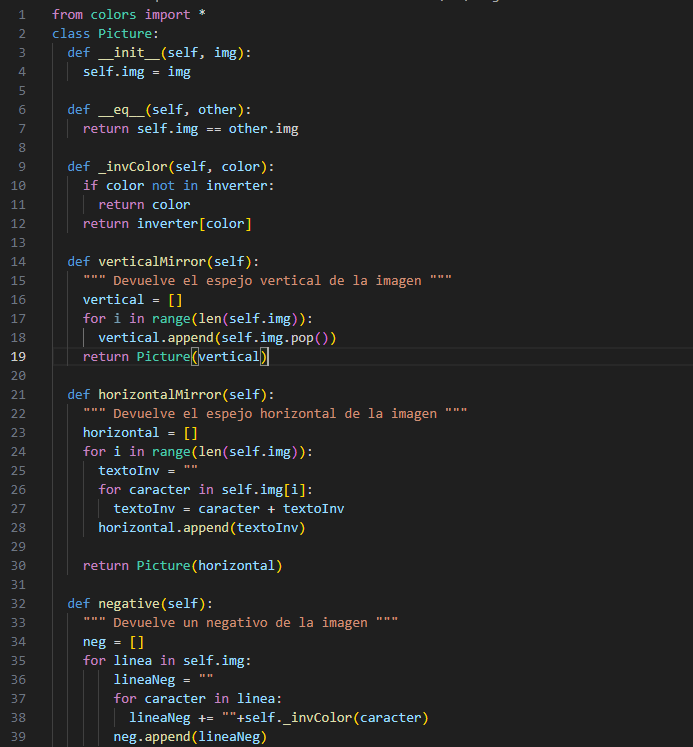
\includegraphics[]{../img/img1.png}
            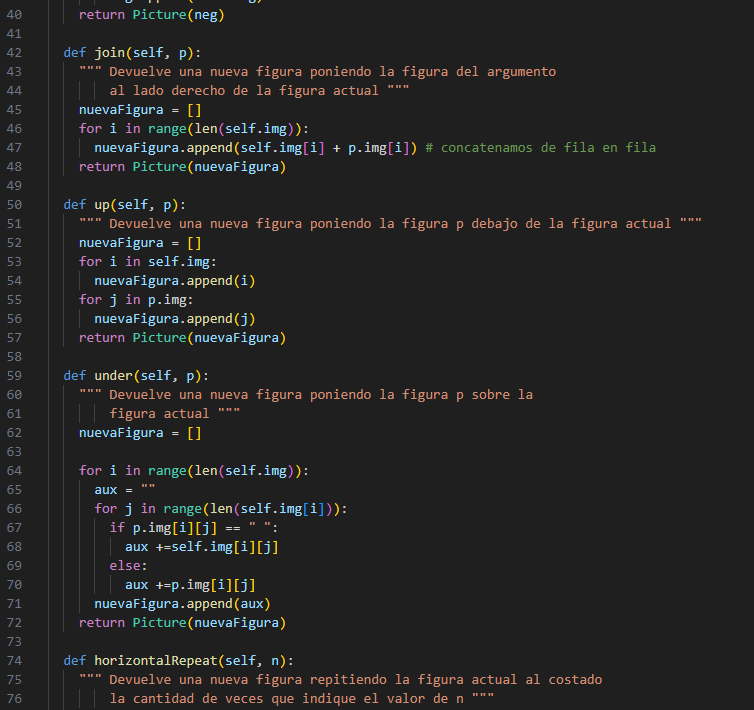
\includegraphics[]{../img/img2.png}\\
            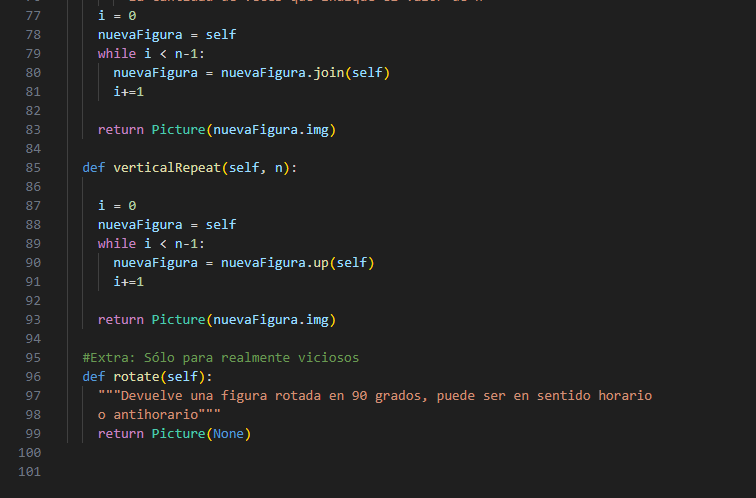
\includegraphics[]{../img/img3.png}\\
            
            \item Ejercicio2a (1): \\
            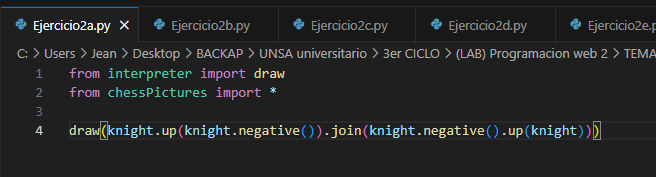
\includegraphics[]{../img/img4.png}\\
            Utilizamos la función negative para hallar el color inverso de nuestra pieza, la función up para colocar
            nuestra pieza arriba de la otra, y la función join para unir estas piezas.
            Colocamos al caballo blanco encima de nuestro caballo negro, una vez realizado esto, la unimos con la otra columna(caballo negro sobre caballo blanco).\\
            Ejecucion:\\
            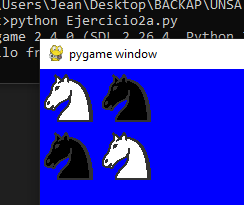
\includegraphics[]{../img/img5.png}\\

            \item Ejercicio2b (2): \\
            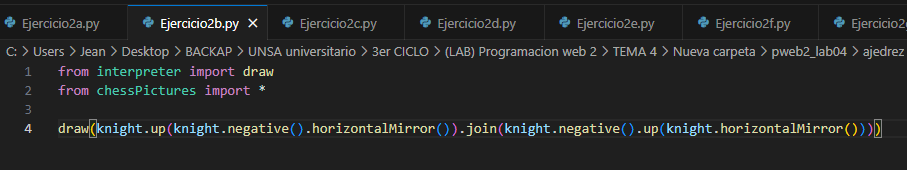
\includegraphics[]{../img/img6.png}\\
            En este ejercicio añadimos la función horizontalMirror(), la cual cambiara de dirección a nuestra
            pieza, haciendo que mire hacia el otro lado. Al igual que el ejercicio2a (1), creamos nuestros
            caballos, los colocamos en columnas y los unimos. \\
            Ejecucion:\\
            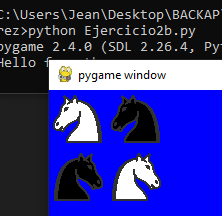
\includegraphics[]{../img/img7.png}\\

            \item Ejercicio2c (3): \\
            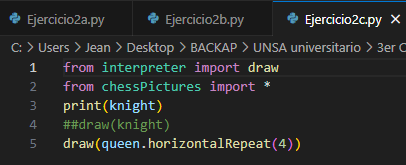
\includegraphics[]{../img/img8.png}\\
            En este ejercicio creamos la función horizontalRepeat, la cual repetirá nuestra pieza un numero
            determinado de veces, esta función concatena a las piezas, haciendo que se coloquen una al costado de otra (izquierda a derecha).\\
            Ejecucion:\\
            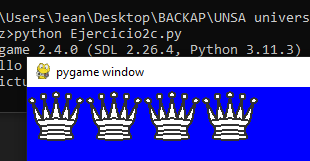
\includegraphics[]{../img/img9.png}\\

            \item Ejercicio2d (4): \\
            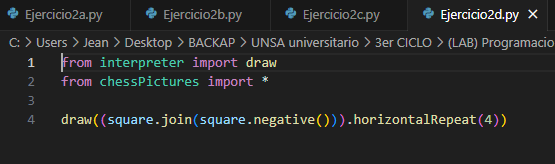
\includegraphics[]{../img/img10.png}\\
            En este ejercicio se nos pide crear una fila de un tablero de ajedrez, por lo que creamos los 2
            primeros cuadrados (blanco y negro) y los repetimos 4 veces, para crear una fila con 8 elementos. \\
            Ejecucion:\\
            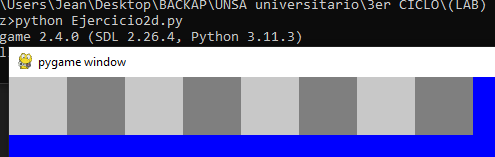
\includegraphics[]{../img/img11.png}\\

            \item Ejercicio2e (5): \\
            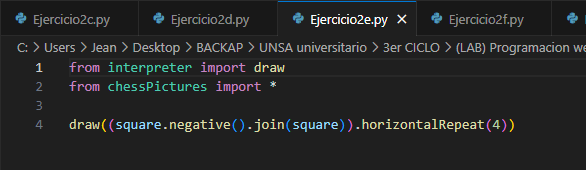
\includegraphics[]{../img/img12.png}\\
            Al igual que el anterior (Ejercicio2d), se nos pide crear una fila de cuadrados, solo que el orden de los cuadrados es diferente (negro y blanco). \\
            Ejecucion:\\
            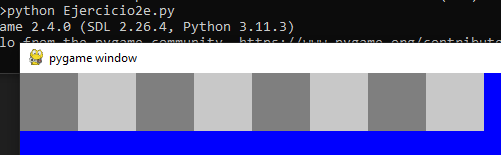
\includegraphics[]{../img/img13.png}\\

            \item Ejercicio2f (6): \\
            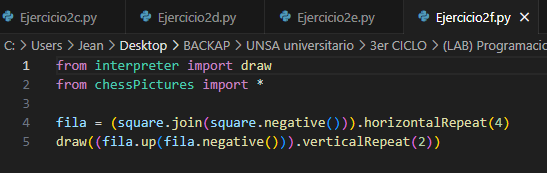
\includegraphics[]{../img/img14.png}\\
            Se crea la función verticalRepeat, la cual al igual que horizontalRepeat, creara varias veces un
            elemento o pieza, pero en columna, es decir, repetirá n veces el elemento hacia abajo.
            En este ejercicio se nos pide crear 4 filas intercaladas de cuadrados, por lo que creamos la variable fila, la cual almacenara una fila intercalada de cuadrados (iniciando con el blanco), luego, lo
            colocamos encima de nuestra fila con color negativo, utilizando la función verticalRepeat, lo
            haremos 2 veces para asi crear 4 filas, puesto que repite 2 veces la creación de 2 filas. \\
            Ejecucion:\\
            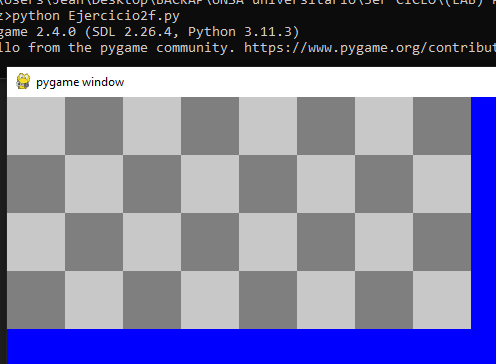
\includegraphics[]{../img/img15.png}\\

            \item Ejercicio2g (7): \\
            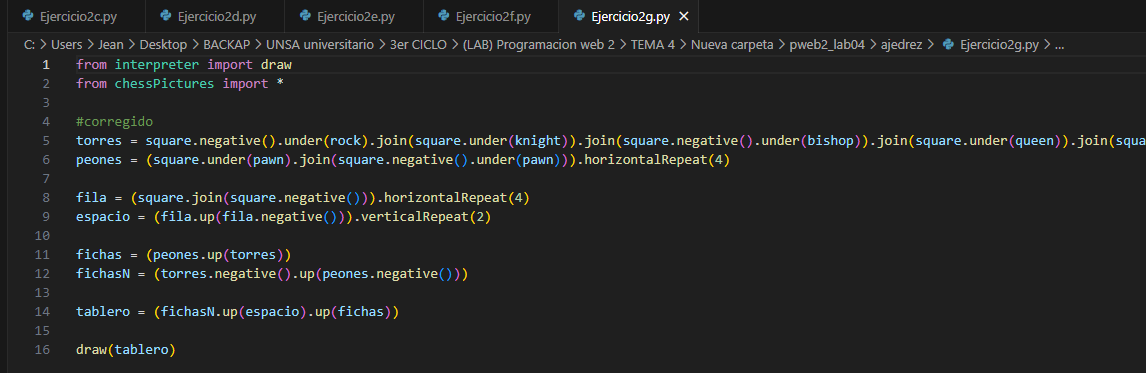
\includegraphics[]{../img/img16.png}\\
            En este ejercicio se nos pide crear un tablero de ajedrez.
            Creamos la variable torres, la cual concatenara con join a todas las piezas en orden de juego, estas
            piezas se encuentran superpuestas a los cuadros respectivos, intercalando de color.
            Seguidamente creamos la variable peones, la cual creara con horizontalRepeat la fila de peones.
            Creamos la variable fila, la cual almacenara una fila de cuadros, repitiéndose 4 veces para llegar a 8 elementos, luego en la variable espacio, la repetimos/ verticalmente 2 veces.
            Creamos las variables fichas y fichasN, las cuales almacenaran el orden de piezas para las fichas
            negras y blancas respectivamente, se utiliza la funcion up y negative para el orden y color.
            Finalmente, unimos las variables en la variable tablero, la cual colocara primero las fichas negras,
            luego el espacio y finalmente las fichas blancas. \\
            Ejecucion:\\
            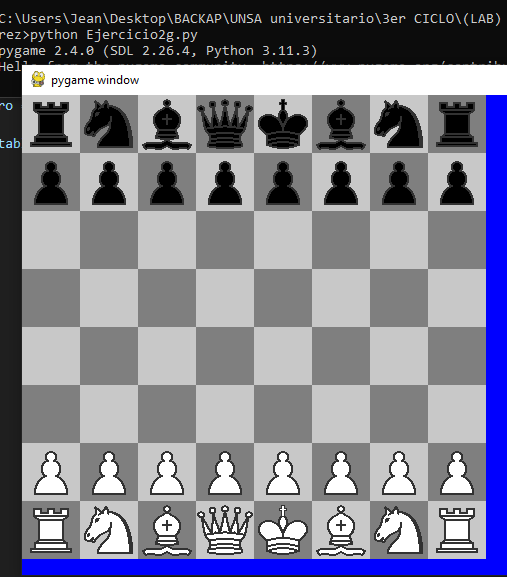
\includegraphics[]{../img/img17.png}\\
            
      \end{itemize}

    \section{Solucion del Cuestionario}
    	\begin{itemize}		
    		\item Explique: ¿Para qué sirve el directorio pycache?
    		\item Almacena el código utilizado por Python para almacenar caché, se utiliza con el propósito de
            aumentar el rendimiento de los scripts.
            Cuando se ejecuta un modulo mas de una vez, en lugar de compilar de nuevo, se busca el caché, en
            caso de encontrarse, se utiliza este mismo para ejecutarse  de forma rápida. 
    	\end{itemize}
    \section{Conclusiones}
    	\begin{itemize}		
    		\item Se utilizo módulos o “librerías” de Python (pygame) para la correcta realización de la práctica. Se ha practicado los temas en Python relacionados a objetos, métodos, funciones, arreglos (listas), ciclos, condicionales, entre otros aspectos básicos con el fin de reforzar nuestro conocimiento del mismo
    	\end{itemize}
    \section{Retroalimentacion general}
    	\begin{itemize}		
    		\item REPOSITORIO GITHUB: \url{https://github.com/JeanChara/pweb2_lab04}
    	\end{itemize}
    \section{Referencias y bibliografias}
    	\begin{itemize}		
    		\item \url{https://docs.python.org/3/library/array.html?highlight=pop#array.array.pop}
    		\item \url{https://docs.python.org/3/tutorial/introduction.html#lists}
    		\item \url{https://docs.python.org/3/glossary.html#term-function}
            \item \url{https://docs.python.org/es/3/tutorial/classes.html}
    	\end{itemize}
     
\end{document}
